\section{Validierung}
Im folgenden Abschnitt wird die Validierung beschrieben. Die Validierung dient zum Auffinden und Beheben von Fehlern, um so eine korrekte Funktion des Programms garantieren zu k�nnen. Zum einen wurden die Berechnungen und Simulationen von Matlab �berpr�ft, zum anderen die Software, aufgeteilt in die Teilbereiche Benutzeroberfl�che und Berechnungen.

\subsection{Matlab}

\subsubsection{Programmierung}
%Problem/Fragestellung:
%- Wie kann die korrekte Funktion der Matlab-Programme �berpr�ft werden?
%L�sung: Die berechneten Antworten werden mit den Antworten von Herrn Niklaus verglichen.
Die Berechnung der Regler wurde zuerst mittels m-Files in Matlab implementiert. Zur �berpr�fung der von Matlab gelieferten Werte wurden diese mit den Werten vom Fachcoach Peter Niklaus verglichen.

\subsubsection{Simulation}
%Problem/Fragestellung:
%- Wie kann die Matlab-Simulation �berpr�ft werden?
%L�sung: Sie wird mit Simulink �berpr�ft.
Mittels Simulink wurde der geschlossene Regelkreis simuliert.

\subsection{Java Software}

\subsubsection{Benutzeroberfl�che}
%Problem/Fragestellung:
%- Wie k�nnen Probleme oder Konflikte bei der Benutzeroberfl�che ausgeschlossen werden?
%Mehrere unabh�ngige User testen die Software.

%Um die einfache Handhabung der Software zu �berpr�fen wurde die Software im ganzen Projektteam sowie von mehreren unabh�ngigen Benutzern getestet. Die so gefundenen Unklarheiten oder Probleme wurden behoben.

\subsubsection{Model}
%Problem/Fragestellung:
%- Wie wird die korrekte Funktion der Software �berpr�ft?
%L�sung: Die Software mit mit JUnit getestet, wobei die Resultate von Matlab erwartet werden.
Die Plausibilit�t der Schrittantworten konnte relativ einfach optisch mit den Graphen �berpr�ft werden, da das Verhalten der einzelnen Regler bekannt ist. Zur genauen �berpr�fung der einzelnen Klassen wurden s�mtliche Klassen des Models mittels JUnit mit den Ergebnissen von Matlab verglichen.

\subsubsection{Performancevergleich Partialbruchzerlegung und IFFT}\label{residuenvsifft}
Es wurde festgestellt dass das Berechnen des Schrittantwortes mittels IFFT-Methode merkbar langsam ist - vorallem dann, als das iterative Approximieren des �berschwingens implementiert wurde, was dazu f�hrte, dass die Schrittantwortberechnung mehrmals ausgef�hrt werden musste.

Durch Reduzieren der Anzahl Punkte kann die Berechnung beschleunigt werden, jedoch kommt dies auf Kosten von Genauigkeit, was in den Figuren \ref{fig:ifft_genauigkeit} zu sehen ist. Weiter sind die Anzahl Punkte bei der IFFT-Methode auf Zahlen der Basis 2 limitiert, was eine genaue Optimierung der Anzahl Punkte unm�glich macht. Durch Ausprobieren stellten wir fest, dass ein Minimum von 4096 Punkte f�r ein visuell genaues Resultat gebraucht wird. Dabei konnten wir auf 2048 Punkte f�r das iterative Approximieren des �berschwingens zur�ckfallen. Die Berechnungszeit war aber immer noch merkbar langsam.

\begin{figure}[h]
\centering
\begin{subfigure}{.4\textwidth}
	\centering
	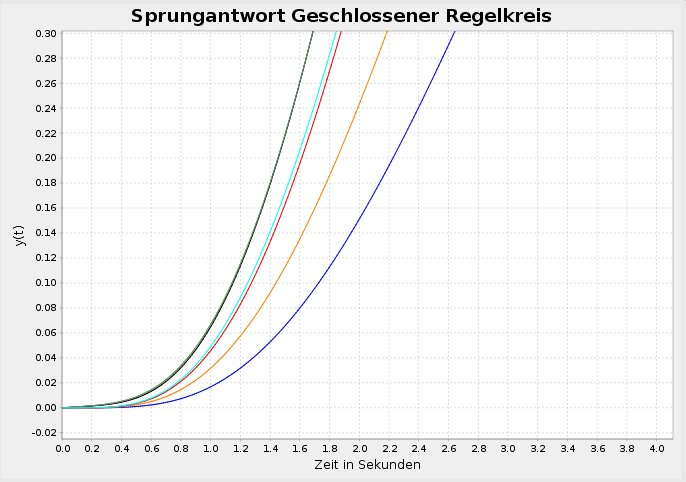
\includegraphics[width=1\linewidth]{./ifft_4096.jpg}
	\caption{Schrittantwort mit 4096 Samples}
	\label{fig:ifft_genauigkeit_4096}
\end{subfigure}
\begin{subfigure}{.4\textwidth}
	\centering
	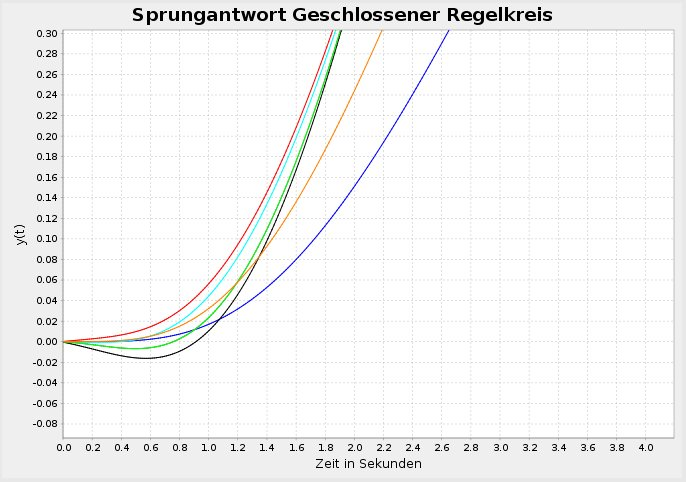
\includegraphics[width=1\linewidth]{./ifft_2048.jpg}
	\caption{Schrittantwort mit 2048 Samples}
	\label{fig:ifft_genauigkeit_2048}
\end{subfigure}
\begin{subfigure}{.4\textwidth}
	\centering
	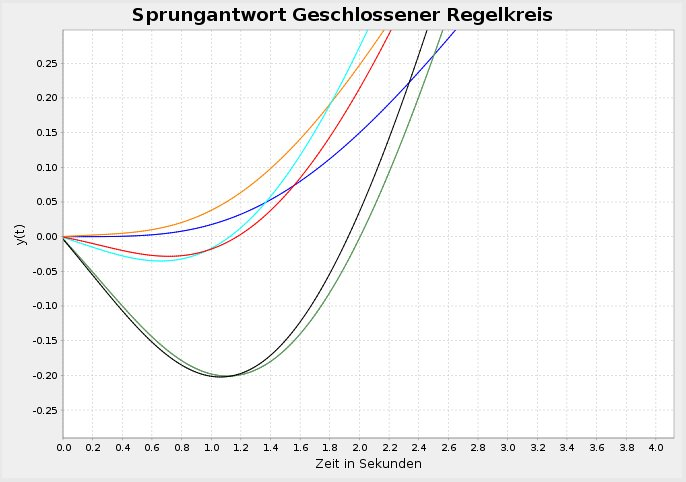
\includegraphics[width=1\linewidth]{./ifft_1024.jpg}
	\caption{Schrittantwort mit 1024 Samples}
    \label{fig:ifft_genauigkeit_1024}
\end{subfigure}
\caption{Vergleich einer Schrittantwort mit verschiedene Anzahl Punkte}
\label{fig:ifft_genauigkeit}
\end{figure}

Es wurde entschieden, eine alternative Berechnungsmethode zu implementieren: Die Schrittantwortberechnung mittels Partialbruchzerlegung.

Um die Berechnungsgeschwindigkeit beider Methoden messen und vergleichen zu k�nnen, wurden mehrere Tests durchgef�rht, welche hier in Detail dargelegt werden.

Die Berechnungszeit wurde mit der Methode \textit{System::currentTimeMillis()} gemessen. Weil die Messresultate stark varieren, wurde die Messung mehrmals mittels einer For-Schleife ausgef�hrt, wie in der Figur \ref{fig:time_measurement_simulate_all} zu sehen ist.

\begin{figure}[h]
	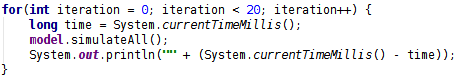
\includegraphics[width=1\linewidth]{./code_for_timing_simulations.png}
	\caption{Zeitmessung der Methode \textit{Model::simulateAll()}}
	\label{fig:time_measurement_simulate_all}
\end{figure}

Wichtig zu bemerkin ist dass das programm f�r jede Messung neu gestartet wurde, damit das \textit{Java Virtual Machine} (JVM) "frish" bleibt.

Die Messungen wurden auf ein System ausgef�hrt mit folgenden Eigenschaften.
\begin{itemize}
	\item \textbf{OS:} Linux twilight 3.18.12-gentoo
	\item \textbf{Arch:} x86_64
	\item \textbf{CPU:} AMD Phenom(tm) II X6 1090T Processor
	\item \textbf{Java:} Oracle JDK 1.8.0.45, Java HotSpot(TM) 64-Bit Server VM
\end{itemize}

